\documentclass[../Head/Main.tex]{subfiles}
\begin{document}
\subsection{Motion planers in action}

The purpose of this test is to find out how well the motion planners work in an actual environment with obstacles. The goal is to lead the robot from an initial position to a target location. 

\subsubsection{Description of test}

The initial position of the robot will be in origo of the environment of the gazebo simulator. Here 14 test of both the tangent bug algorithm and model based planner will be conducted for the 14 rooms of the \textit{bigworld} map. The idea is to test the success rate of finding rooms, the robots distance to the closest obstacle on the path to the goal and the distance travelled along the way. The model based planer will be tested with a higher speed than the tangent bug algorithm because it will be further away from obstacle most of the time and thereby less likely of hitting obstacles.           

\subsubsection{Test parameters}

\begin{tabular}{l r}
	- World used                & bigworld\\	
	- Speed of tangent bug      & -1 to 1\\
	- Speed of model planer     & -2 to 2\\
	- Number of tests           & 14
\end{tabular}

\subsubsection{Data}
\subfile{../Tables/Dist_travelled_and_dist_to_obstacle_modelbased}
\subfile{../Tables/Dist_travelled_and_dist_to_obstacle_tangent_bug}
\subfile{../Figures/Graphs_dist_to_obstacle}
\subfile{../Figures/Comparason_motion_planners}

\begin{figure}[H]
	\centering
	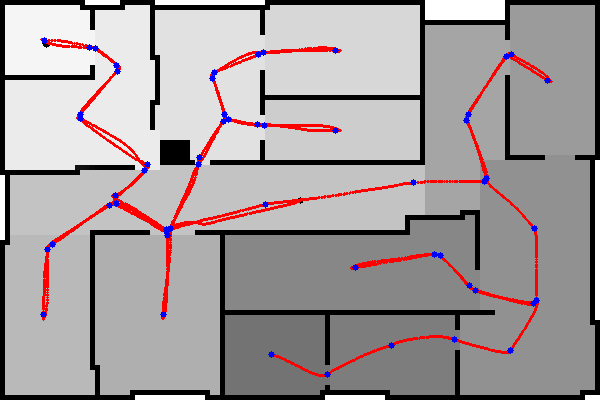
\includegraphics[width=0.6\textwidth]{Modelbased/brushfireTest15}
	\caption{Illustration of the run visiting all rooms starting from the origin for the model based planner}
	\label{fig:Test15}
\end{figure}

\subsubsection{Conclusion}

\end{document}